%---
\section{Project Management}
\label{sec:ProjectManagement}

%{\bf\color{red}
%Si richiede di descrivere la strategia di progetto attraverso gli strumenti di Project Management come per esempio il Project Management Plan e si richiede inoltre di presentare uno schema riassuntivo sulle tipologie delle gare d’appalto necessarie per la realizzazione dell’Esperimento (LNGS tender, INFN tender, European tender) includendo tempi e risorse stimate per il suo espletamento.

% In particolare si chiede di esplicitare i seguenti strumenti:
%\begin{itemize}
 %   \item \underline{Fasi del Progetto, Individuazione e descrizione delle principali fasi di un esperimento}: e.g. APPROVAL – DESIGN - BUILDING – COMMISSIONING – OPERATION \& MAINTENANCE – UPGRADE - DECOMMISSIONING
  %  \item \underline{Work Breakdown Structure:} Redazione dello schema della WBS e descrizione dei Work Packages. 
   % \item \underline{Schedule:}
    %\item \underline{Budget:} Elaborazione della tabella dei costi di progettazione, costruzione, installazione, operazione e smantellamento individuando anche il budget di contingency e specificando i costi relativi per l’adeguamento impiantistico e strutturale dei LNGS. Elaborazione di un Cost Breakdown Structure secondo lo schema allegato.
    %\item \underline{Risks:} Compilazione della Matrice e del registro dei rischi, secondo lo schema allegato.
%    \item \underline{Organizational Breakdown Structure}
 % Elaborazione dell’Organizzazione del progetto includendo i ruoli e le responsabilità (OBS).
  %  \end{itemize} 
%}

%\vspace{1cm}

A detailed Project Execution Plan (PEP), prepared for the NSF Mid Scale funding Request in May 2019 is attached to this document. In that document all the project organization and management tools are described as well as the current Work Breakdown Structure and Gantt chart. Details on the funding scheme and institution responsibility and cost sharing is also reported there. We refer to the attached document for all aspect mentioned before. In the following only relevant additions  are reported.

%\subsection{Update with respect to the attached PEP}
%\begin{enumerate}
%\item Updated general Gantt chart and relevant discussions.
%\item Compilation of the risk register (example below from LNGS template).
%\item Costs including operations and dismantling and costs relative to  LNGS infrastructure upgrade and their sources.
%\end{enumerate}

%\begin{figure}
%\begin{center}
%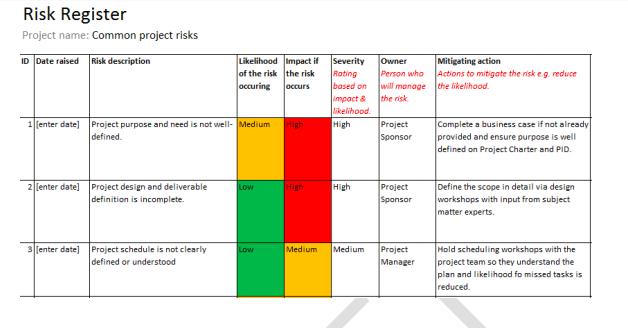
\includegraphics[width=\textwidth]{./Figures/RiskRegisterLNGSTemplate}
%\caption{Preliminary Risk Registry Table for \DSk project(from LNGS teamplate}
%\label{fig:RiskRegistry}
%\end{center}
%\end{figure}

%\begin{figure}
%\begin{center}
%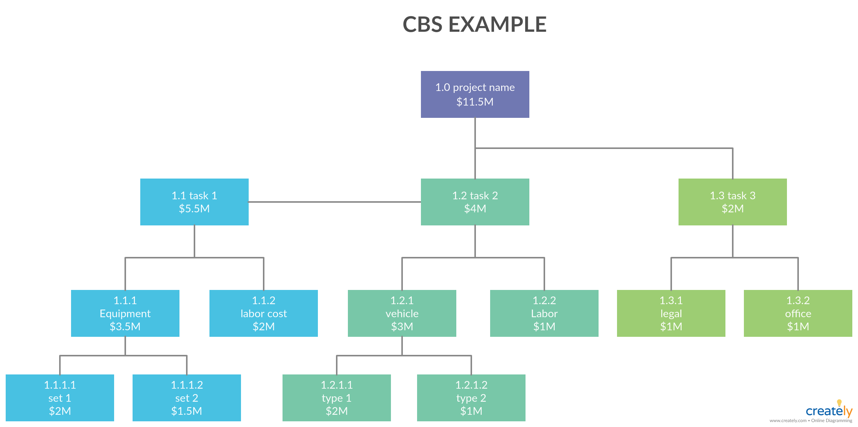
\includegraphics[width=\textwidth]{./Figures/CostBreakdownStructureLNGSTemplate.png}
%\caption{Cost Breakdown Structure for \DSk project (from LNGS teamplate}
%\label{fig:CostBreakdownStructure}
%\end{center}
%\end{figure}
